\documentclass[conference,harvard,brazil,english]{sbatex}
\usepackage[utf8]{inputenc}
\usepackage{ae}
%
% LaTeX2e class SBATeX
%
%
% Versão para Overleaf 
% Diego Eckhard
% diegoeck@ufrgs.br
%
%
% Versão 1.0 alpha
%   Walter Fetter Lages
%   w.fetter@ieee.org
%
% Este arquivo sbai2013.tex é uma adaptação do arquivo revista.tex,
% Versão: 1.0 alpha, desenvolvido por Maurício C. de Oliveira,
% mcdeoliveira@ieee.org.
%
% As adaptações fazem com que, por default, sejam utilizadas
% as opções adequadas para o formato do SBAI 2017.
% --------------------------------------------------
%  Estes comandos são necessários apenas para a
%  a geração deste artigo exemplo. Eles não fazem
%  parte do estilo SBATeX.
% --------------------------------------------------
\makeatletter
\def\verbatim@font{\normalfont\ttfamily\footnotesize}
\makeatother
\usepackage{amsmath}
% --------------------------------------------------

\usepackage{graphicx}
\usepackage{float}

\usepackage[lined,ruled,boxed]{algorithm2e}
%\usepackage{algorithmic}



\usepackage[table]{xcolor}
\usepackage{booktabs}

\usepackage{caption}
\usepackage{subcaption}
%\usepackage{hyperlinks}
\usepackage{url}


%-----------------------
\usepackage{mathtools, nccmath}
\newcommand{\N}{\mathbb N}
\newcommand{\Q}{\mathbb Q}
\newcommand{\R}{\mathbb R}

\usepackage{xparse}
%
\DeclarePairedDelimiterX{\set}[1]{\{}{\}}{\setargs{#1}}
\NewDocumentCommand{\setargs}{>{\SplitArgument{1}{;}}m}
{\setargsaux#1}
\NewDocumentCommand{\setargsaux}{mm}
{\IfNoValueTF{#2}{#1} {#1\,\delimsize|\,\mathopen{}#2}}%{#1\:;\:#2}

\parindent = 0pt

\usepackage{amsfonts}
\newcommand{\commentib}[1]{{\color{blue} [IB: #1]}}

\newtheorem{myDefinition}{Definition}

\begin{document}

% CABEÇALHO

\title{PLANNING AND EVALUATION OF UAV MISSION FOR INTRALOGISTICS PROBLEM}

\author{Thiago R. F. Cavalcante}{thiagorodrigoengcomp@gmail.com}
\address{Graduate Program in Electrical Engineering, Federal University of Amazonas, Manaus, AM, Brazil}

\author{Iury V. de Bessa}{iurybessa@ufam.edu.br}
\address{Department of Electricity, Federal University of Amazonas, Manaus, AM, Brazil}

\author{Lucas C. Cordeiro}{lucas.cordeiro@cs.ox.ac.uk}
\address{Department of Computer Science, University of Oxford, Oxford, United Kingdom}



% \twocolumn apenas para conference
\twocolumn[

\maketitle

\selectlanguage{brazil}
\begin{abstract}
Este artigo apresenta o desenvolvimento de planejadores de missão na intralogística para um veículo aéreo não tripulado comercial, equipado com uma garra robótica, em um ambiente industrial onde há almoxarifado de insumos, linhas de produção e deposito de produtos. Neste trabalho, o planejador gera comandos necessários para realizar uma missão a qual compreende desde a entrega de insumos trazidos do almoxarifado à linha de produção, até a entrega do produto final ao cliente. Foram desenvolvidas duas abordagens diferentes para planejamento de missão: na primeira abordagem, utilizou-se uma simples heurística que resolve o problema, onde o VANT leva os insumos do almoxarifado para a respectiva linha de produção e fica esperando a produção terminar, por um período de tempo característico de cada linha de produção; já na segunda abordagem, utilizou-se uma técnica com escalonamento de tarefas (processo de produção). Estas abordagens seguem algumas regras de produção que serão apresentadas ao longo deste trabalho. Foi realizado uma avaliação dos planejadores de missão desenvolvidos, verificando o custo de ambos, realizando algumas medidas de tempo de execução, bem como comparando estes resultados com o custo ótimo obtido  com a ferramenta de otimização CPLEX.   \end{abstract}

\keywords{Planejamento de Missão, Sistemas de Manufatura, Problemas de Otimiza\c{c}\~ao.}

\selectlanguage{english}
\begin{abstract}
This paper presents the development of mission planners in intralogistics for a commercial unmanned aerial vehicle equipped with a robotic gripper in an industrial environment, which consists of an input warehouse, production lines, and a product warehouse. In this study, the planner produces the needed commands for carrying out a given mission, which includes the delivery of inputs brought from the warehouse to the production line until the final product is delivered to the customer (product warehouse). Two different approaches are developed for mission planning: in the first approach, a simple heuristic is used to solve the mission problem, where a UAV gets the necessary inputs to produce a product, from the warehouse, and bring to the respective production line and the UAV waits in production line site to finish the production of the product; in the second approach, a technique with task scheduling (production process) is employed; both approaches follow a set of production rules. An evaluation of the developed mission planners is performed, verifying the cost of both approaches, measuring the execution time, and comparing those results with the optimum cost obtained with the IBM ILOG CPLEX optimizer.
\end{abstract}
\keywords{Mission Planning, Manufacturing Systems, Optimization Problems.}
]

% CONTRIBUIÇÃO
\selectlanguage{english}

\section{Introduction}
\label{sec:introduction}

% Use of a commercial UAV - 3DR IRIS + in the intra-logistics, {\it i.e., Internal Logistics of movement and storage.}, aiming to give another option of agility in the manufacturing process. Additionally, it will be approached a study of evaluation of the cost of the missions that the UAV executes in this process.

Logistics has become a competitive and fundamental factor for organizations, involving the management, conservation, and supervision of freight transport. In addition, excellent logistics means customer satisfaction; so speed is still an important factor in a successful logistics process~\cite{drone4logistic}. Currently, one of the solutions to this type of problem is the use of unmanned aerial vehicles (UAVs). Nowadays, UAVs are mostly remotely piloted vehicles (RPV), since their operations are carried out by ground operators. If the tasks performed by a UAV are performed autonomously, it would relieve the work of these operators, since they perform tedious and repetitive tasks~\cite{pascarella2013autonomic}.

One possible improvement of these logistics systems is the increase of the UAVs automation, which results in costs minimization. Consequently, investments and studies related to stand-alone UAVs are important to the smart factories development~\cite{hern2014dhl}. However, one of the main problems for using autonomous UAVs is the system's reliability and intelligence. Thus, increased employment of autonomous UAVs requires the development of devices, which are able to perform tasks and interact with the environment in an intelligent and reliable way.

Autonomous UAVs need to know what will happen in a future instant and what is the best decision to make at the present time; therefore, they require strategies not only to decompose their missions into meaningful sub-tasks, but also to track progress toward mission goals and the evolution of these tasks relative to the autonomous UAVs capabilities~\cite{finn2012developments}. As a consequence, in order to successfully perform a mission, it is recommended to perform task planning~\cite{finn2012developments}. Mission planning problems consist of planning events to meet certain requirements and objectives~\cite{krozel1988search}. Therefore, this \commentib{this o q??} is one of the main challenges faced in solving this problem.

Both academy and industry have done researches about evaluation and optimization of mission planning in the last years. \citeasnoun{schwarz2012towards} have used ant colony to optimize missions for an automated guided vehicle (AVG). Another paper investigates energy consumption for a factory and evaluates the logistic planning processes using statistical metrics of evaluation~\cite{muller2012analyzing}.

%\textcolor{red}{Is there some related work that solves the problem? You have to describe here...}

To evaluate mission planning strategies, evaluation metrics must be employed. An evaluation metrics consists of a set of measures that follow a common underlying evaluation methodology. It is used to evaluate the efficacy of information retrieval systems and to justify theoretical and/or pragmatical developments of these systems \cite{pehcevski2009evaluation}. In this work, we use an optimal measure to compare with a calculated value of a mission cost.

This paper presents a methodology that evaluates the cost of mission planners for a commercial UAV. We developed an evaluation metrics that evaluates the relative cost of a planning strategy related with the optimal cost generated by the CPLEX optimizer \cite{cplex2003ilog}. %The evaluation is made by comparing the mission execution time with the cost of an optimal solution solved by CPLEX solver. Additionally, a middleware was developed to interface the mission planning application and the embedded control software, adapting the UAV for intra-logistics. Finally, experiments were done to verify the consistency of evaluation methodology.

In summary, the main contributions of this study are:
\begin{itemize}
\item a novel evaluation methodology for UAV intralogistics mission planners algorithms, which allows predicting the planners performance and also obtaining optimal algorithms and missions;
\item development of an intralogistcs mission planner framework that provides mission commands for a UAV system; 
\item use of a commercial UAV system in intralogistics missions to demonstrate the evaluation methodology efficiency.
\end{itemize}

As a result to this work, we have verified that the development and experiments of the mission planner evaluation methodology were done successfully as sown in Section~\ref{sec:results}. Additionally, the framework to command and control a UAV was gratefully developed and tested in simulated and real environment.

\textit{Outline}. Section~\ref{sec:related} shows previous studies related to mission planning, optimization, and evaluation. Section~\ref{sec:background} provides the fundamentals of mission planning and optimization problems. Section~\ref{sec:uav} describes the UAV movement system used in this work. Section~\ref{sec:method} explains the proposed evaluation methodology in further details. Section~\ref{sec:results} describes the experimental procedures and results in order to explore and demonstrate the potential of methodology, and, finally, Section~\ref{sec:conclusao} concludes this study and describes future work.

%%%%%%%%%%%%%%%%%%%%%%%%%%
\section{Related Work}
\label{sec:related}
%%%%%%%%%%%%%%%%%%%%%%%%%%

In the literature, there are attempts to implement UAV guidance systems that perform mission planning. \citeasnoun{doherty2009temporal} presented a framework architecture for mission planning and execution tracking applied to an unmanned helicopter. During the mission execution, knowledge is acquired through sensors, which was used to create state structures. These structures allow constructing a logical model, representing the real system development and its environment over time. Then, the planning and monitoring modules use temporal action logic (TAL) to reason about actions and changes.

The NASA/U.S. Army autonomous helicopter project has developed a guidance system for the autonomous surveillance planning problem for multiple and different targets~\cite{whalley2005design}, which generates mission plans using a theoretical approach for decision making. A high-level standalone control is provided by the framework Apex~\cite{baer1998nasa}, a reactive procedure-based scheduler/planner used to perform mission-level tasks. Apex synthesizes a course of action primarily by linking elemental procedures expressed in procedural definition language (PDL), a notation developed especifically for the Apex reactive planner. This guidance system is integrated into a robotic helicopter and tested in more than $240$ scenarios.

A similar project, called Ressac (Research and Rescue by Cooperative Autonomous System), is conducted by the French Aerospace Laboratory (ONERA) for a search and rescue scenario~\cite{fabiani2007autonomous}. This architecture for an exploration mission is developed based on the idea of decomposing the mission into a sequence of tasks or macro-actions associated with rewards. The problem is modeled using a Markov decision process framework (MDP) and dynamic programming algorithms for mission planning. Konigsbuch~\cite{teichteil2007multi} extends the guidance system and integrates with a robotic helicopter.

Finally, the German Aerospace Center (DLR) has also developed a mission management system based on the behavior paradigm~\cite{adolf2010onboard}, which has been integrated with the ARTIS helicopter and validated in different scenarios, including waypoints follower, search and tracking mission.

Existing approaches for evaluation of mission planners for intralogistics problems are either empirical or theoretical. This paper describes an approach combining both aspects. In addition, we test the metrics in a real environment, \textit{i.e.}, we use a real UAV to perform a mission and we measure the cost (mission execution time) of the mission.

\textcolor{red}{Are you sure that there is no related work that solves the problem? Please double-check in the Scopus digital library!}
%--------------------------------------------
\section{Preliminaries}
\label{sec:background}
%--------------------------------------------

%--------------------------------------------
\subsection{Terminology}
\label{sec:terms}
%--------------------------------------------

Key definitions related to the case study and the application developed in this study need to be clarified. All definitions below are adopted in the remainder of this study.

\begin{myDefinition} 
\textbf{(Mission Command)} 
Mission Command is a command created to execute a task such as to go from one location to another, get a package using a robot gripper, and land a UAV.
\label{def:missioncommand}
\end{myDefinition}

\begin{myDefinition}
\textbf{(Mission)} 
Mission is the set of steps and mission commands that the UAV executes to produce the customer's order.
\label{def:mission}
\end{myDefinition}

\begin{myDefinition}
\textbf{(Warehouse)}
Warehouse is the set of stored raw material available until the moment of entering the productive process. The raw materials, i.e., the inputs available in this work are inputs A, B, and C.
\label{def:almoxarifado}
\end{myDefinition}

\begin{myDefinition} 
\textbf{(Order)}
Order is the requisition of products made by the client. In this study, the products are of type X and Y.
\label{def:pedido}
\end{myDefinition}

\begin{myDefinition}
\textbf{(Production Time)}
Production time is the time required to produce a product X or Y, after making available all the needed inputs for the production, given by the production rule.
\label{def:tempoProducao}
\end{myDefinition}

\begin{myDefinition}
 \textbf{(Production Rule)}
Production rule describes what and how many inputs are needed to produce a particular product.
\label{def:regraProducao}
\end{myDefinition}

\begin{myDefinition}
\textbf{(Mission Planner)}
Mission planner is the agent who performs the planning of a mission, that is, produce all steps and commands needed to carry out a given mission.
\label{def:planejadorMissao}
\end{myDefinition}

\begin{myDefinition}
 \textbf{(Mission File)}
The mission file is a file that is created for the context of this work, with the extension \textsc{.mission} containing the mission itself.
\label{def:arquivoMissao}
\end{myDefinition}

\begin{myDefinition}
 \textbf{(Movement Function)}
The movement function are functions created in Python using the drokekit API to send commands to the UAV by MAVLink protocol.
\label{def:movFunc}
\end{myDefinition}

\begin{myDefinition}
 \textbf{(Production Mission)}
The production mission is the set of steps to produce all the product required by the client.
\label{def:prodMission}
\end{myDefinition}


%--------------------------------------------
\subsection{Mission Planning}
\label{subsec:missionplanning}
%--------------------------------------------

Firstly, a mission can be defined as a goal that needs to be completed (cf. Definition~\ref{def:mission}). In the context of this study, the UAV mission is the packages delivery according to a set of well defined rules. A definition to mission planning for UAV is the process of planning the locations to visit (waypoints) and the actions that the vehicles can perform (e.g., loading/dropping a load and taking videos/pictures), typically over a time period~\cite{ramirez2014solving}. Functionally, mission planning lies above the trajectory planning process, where the mission planner (cf. Definition~\ref{def:planejadorMissao}) generates a desired mission plan, and then the trajectory planner generates the flight plan (trajectories) between the waypoints.

%\subsubsection{Related Works in Mission Planning}



%\subsection{UAV Navigation}
%--------------------------------------------
\subsection{Optimization Problems}
%--------------------------------------------

An optimization problem is related to finding the best solution (relative to a certain criterion) among a set of available alternatives. For instance, the popular bin packaging problem that aims to find the number of boxes of a certain size to store a set of objects of indicated sizes; optimization involves, for example, finding the least amount of boxes. An optimization problem is usually represented as follows:

\begin{equation}
	\label{eq:optproblema}
	\begin{array}{cc}
		\min & f(\textbf{x}),  \\
		\textrm{ s.t. } & \textbf{x}\in\Omega.\\
	\end{array}
\end{equation}	

\noindent where $\Omega$ is a set of the problem constraints and $f(x)$ is the function to optimize.
	
An optimization problem can be defined as a finite set of variables, where the correct values for the variables specify the optimal solution. If the variables are of the set of real, the problem is called continuous, and if they can only have a finite set of distinct values, the problem is called combinatorial~\cite{korte2012combinatorial}.

%Two distinctions need to be made to better understand the universe of optimization problems. The first is to distinguish a problem which refers to a more general class, for example, the problem of packaging, and an example representing a special type of problem, for example the problem of packaging, wherein there are 5 packages for packaging 25 objects of different sizes. The second distinction concerns the existence of two categories of problem classes: the abstract problem classes and the concrete problem classes. As the name itself suggests, the second category refers to problems that have "concrete existence," that is, problems for which instances can be created. The BPP corresponds to this category. Together they are also part of a more abstract class: grouping problems. Only with the problem of abstract classes, it is impossible to define instances. In fact, as shown in Figure~\ref{fig:problemasDeOtimizacao}, the classes of concrete and abstract problems form a hierarchy of optimization problems.
%
%\begin{figure*}[h]
%	\centering
%	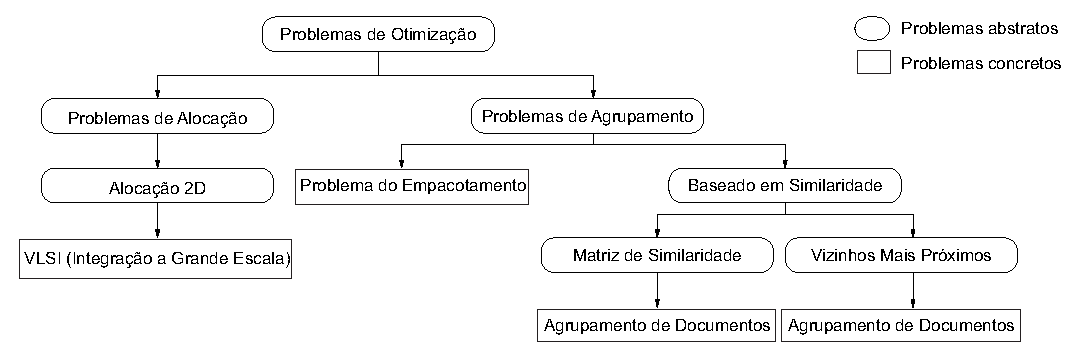
\includegraphics[width=1.0\textwidth]{problemasDeOtimizacao.eps}
%	\caption{Some Optimization Problems.\commentib{Falta apenas traduzir a imagem.} \label{fig:problemasDeOtimizacao}}
%	\end{figure*}
%	
%	An optimization problem can be defined as a finite set of variables, where the correct values for the variables specify the optimal solution. If the variables are of the set of real, the problem is called continuous, and if they can only have a finite set of distinct values, the problem is called combinatorial \protect\cite{francq2011optimization}.
%	
%	In order for the optimization problems to be solved, it is necessary to develop a method that solves them, which are the algorithms. An important category of problems are the NP-hard problems, where they can only be solved by certain algorithms that try to arrive at the optimal solution of that determined problem.
%	
%	When the optimal solution of an NP-hard problem is not guaranteed, this type of method is called a heuristic. A heuristic is an intuitive way of solving a particular problem, where the best possible solution is not guaranteed.
%	
%	Every optimization problem is basically characterized by having an objective function, which can be called cost function when it is desired to minimize it or utility function when it is desired to maximize it, and a set of constraints that delimit the space of viable solutions, or Be the region where the solutions are that can be accepted. The objective function contains a set of variables to which values must be assigned in a systematic way so as to walk through the search space and find the one that optimizes the result to be searched, in case a maximization problem finds the highest possible value while in a Minimize the value. In both cases the solution must satisfy the set of constraints imposed to be accepted. 


%	One can interpret the space of solutions as being a subset of Euclidean space \(\R^n\). Each variable is a dimension of space. For a function with two variables it is possible to form in a two-dimensional space and with the addition of a third dimension to the result of the function with \(x\) and \(y\) as input it is possible to observe the behaviour of the function as The \(x\) and the \(y\) of the function undergo variation. In Figure ~\ref{fig:sol} a two-dimensional graph is shown in which the variation of the function value causes changes in the gray scale. For larger values ??a darker gray is obtained and for smaller values ??a lighter gray is obtained. With this, one can observe the space of solutions in a panoramic way in the two-dimensional space and it is verified that as it approaches the center the function generates smaller values. In it it is also possible to notice that the x-shaped marks, which represent the solutions found, vary towards the local minimum that is in the middle of the search space. The heuristic used to search for the optimal solution in this case was to look for neighbouring solutions that minimized the cost of the function in the same way that a sphere that rolls over an inclined plane stabilizes when it reaches a valley that would be the local minimum Function. However, this heuristic is not always the most adequate, as will be seen later.
%
%\begin{figure}[H]
%	\centering
%	\includegraphics[width=0.5\textwidth]{sol.eps}
%	\caption{Walking through the space of solutions\label{fig:sol}}
%\end{figure}

%%%%%%%%%%%%%%%
\section{UAV Movement System}
\label{sec:uav}
%%%%%%%%%%%%%%%

% \subsection{UAV Movement System}

%In this section, we first investigate the UAV platform used (3DR IRIS+) in this study, describing the hardware characteristics and the control framework developed for intralogistics missions. 
The core hardware of the UAV IRIS+ is the Pixhawk and we can control it using a Python library \cite{dronekit}, which uses Micro Air Vehicle Link (MAVLink) protocol~\cite{meier2011pixhawk}. MAVLink is a protocol for communicating with small unmanned vehicle, which is designed as a header-only message marshalling library.

The IRIS+ UAV is integrated into a robot gripper to take and leave packages during missions (cf. Definition~\ref{def:mission}). We have connected a servo motor to the Pixhawk by one of the pulse width modulation (PWM) outputs. Figure~\ref{fig:hardArch} shows the system hardware architecture and the interconnections between each component module. In the hardware architecture shown in the Figure~\ref{fig:hardArch}, we can see the UAV hardware component connections where there is the Pixhawk (flight controller) and its connections between other componeeents such as the compass, GPSPWM outputs, battery and etc. Moreover, it shows the connection with a robot gripper using a PMW outupts as a signal control for the servo motor in the robot gripper. Finally, it shows the communication between a personal computer (PC) and the UAV via radi control (RC) signal.
%
\begin{figure}[H]
	\centering
	\includegraphics[width=\columnwidth]{arquiteturaIHW.eps}
	\caption{System Hardware Architecture.}
	\label{fig:hardArch}
\end{figure}

In the software architecture, the Mission Planner (cf. Definition~\ref{def:planejadorMissao}) reads the warehouse inputs and client order and produces a \texttt{.mission} file, which contains the list of mission commands needed for producing the required client order. This \texttt{.mission} file is used by a UAV Control Program to control the UAV and to produce the low-level movement commands using MAVLink protocol (cf. Definition~\ref{def:missioncommand}). Figure~\ref{fig:sysArch} shows the mission planning framework software components.


In order to control the UAV from a PC, we have used the dronekit API that translates MAVLink commands to a Python function. In the ground station, the PC is running the UAV Control Program that controls the UAV using a radio module connected to the PC via USB. We have created a bunch of functions in the control program for the most common UAV actions. The movement functions (cf. Definition~\ref{def:movFunc}) are described in Table~\ref{table:movfunc}.
%
%\begin{itemize}
%\item \texttt{TakeOff}: takeoff command of the UAV;
%\item \texttt{GoTo}: command to move the  UAV to a certain location;
%\item \texttt{TakePackage}: command to collect an input/product through a robot gripper;
%\item \texttt{LeavePackage}: command to leave an input or product from a robot gripper;
%\item \texttt{Wait}: command to make a UAV to hover (wait);
%\item \texttt{Land}: command to make a UAV to land.
%\end{itemize}

\begin{table}[]
\scriptsize
\centering
\caption{Description of movement functions}
\label{table:movfunc}
\begin{tabular}{|l|l|}
\hline
\multicolumn{1}{|c|}{\textbf{Command}} & \multicolumn{1}{c|}{\textbf{Description}}           \\ \hline
\texttt{TakeOff}                     & takes off the UAV                                   \\ \hline
\texttt{GoTo}                        & moves the UAV to a certain location                 \\ \hline
\texttt{TakePackage}                 & takes an input/product (gripper) \\ \hline
\texttt{LeavePackage}                & leaves an input/product (gripper)   \\ \hline
\texttt{Wait}                        & makes the UAV to hover (wait)                       \\ \hline
\texttt{Land}                        & lands the UAV                                       \\ \hline
\end{tabular}
\end{table}


\begin{figure}[H]
	\centering
	\includegraphics[width=0.8\columnwidth]{sysArch.eps}
	\caption{System's Architecture.\label{fig:sysArch}}
\end{figure}


%\subsection{Mission Planning}
%\label{mission}


%%%%%%%%%%%%%%%
\section{Methodology of Time Cost Evaluation, UAV Use and Mission Planning}
\label{sec:method}
%%%%%%%%%%%%%%%

%\commentib{Modifique o t\'itulo (expanda). Metodologia de qu\^e?? Tente fazer algo parecido com o do trabalho.}

%In this section, we evaluate the algorithm mission cost and describe a case study to a UAV and contents about mission planning.

%%%%%%%%%%%%%%%%%%%%%%%%%%%%%%%%%%%%%
\subsection{Case Study: UAV Intralogistics Mission}
\label{sec:ec}
%%%%%%%%%%%%%%%%%%%%%%%%%%%%%%%%%%%%%

In order to model the mission planning problem as an optimization problem, the case study shown in Figure~\ref{fig:useCase} is used.
%
\begin{figure}[ht]
	\centering
	\includegraphics[width=0.7\columnwidth]{useCase.eps}
	\caption{Case Study Representation.\label{fig:useCase}}
\end{figure}
	
Figure~\ref{fig:useCase} shows that there are three types of inputs in the warehouse (i.e., A, B, and C) and two production lines that produce two different products (i.e., X and Y). Each production line produces only one type of product and has a characteristic production time (cf. Definition~\ref{def:tempoProducao}). Figure~\ref{fig:useCase} shows that to produce a product of type X, two inputs of type A and one input of type C are required, and to produce a product of type Y, two inputs of type B and one input of type C are required. The production time of a X product is $4 p.u.$ and the time of production of product Y is $6 p.u.$. A production unit ($1 p.u.$) is considered to be a \texttt{GoTo} command performed by the UAV.

The task to be performed is the production of the client order (cf. Definition~\ref{def:pedido}), where a given UAV collects supplies from the warehouse, takes that to the production line, and once the production of a certain product is finished, the UAV delivers it to the client.

%%%%%%%%%%%%%%%
\subsection{Modelling a UAV Intralogistics Mission as an Optimization Problem }
\label{ssec:modelo}
%%%%%%%%%%%%%%%

The purpose of this subsection is to make the mission planning problem into an optimization problem, creating a modelling for the problem; in order to find, afterwards, the shortest execution time of all tasks (minimization), based on the case study explained in Section~\ref{sec:ec}. The notation used is given below:

\begin{itemize}
\item $\mathcal{T} = \set{T_j \vert j\in \mathbb{N}^{*},j\leq N}$ is the set of $N$ tasks;
\item $\mathcal{M} = \set{m_i \vert i\in \mathbb{N}^{*},i\leq M}$ is the set of $M$ production lines (machines);
\item $\mathcal{P} = \set{p_j \vert j\in \mathbb{N}^{*},j\leq N}$ is the processing time of each $j$-th task;
\item $S = \set{s_i \vert s\in \mathbb{N}^{*},i\leq M}$  is the setup (production) time of each $i$-th production line;
%\item $R||C_{max}$ (Three-field notation\footnote{Notation $\alpha | \beta | \gamma$, where $\alpha$: processing environment, $\beta$: problem constraints and $\gamma$: optimization criterion.} used in the literature to represent a given task scheduling problem, in this case, minimizing the makespan \footnote{Makespan is the termination time of the most loaded processor.\label{nt:makespan}} in an unrelated parallel machine environment \cite{graham1979optimization}.
\end{itemize}

\paragraph{Decision variable}

The variable $x_{ij}$ is a binary decision variable that takes the value $1$ if the task $j$ is running on the machine $i$; and $0$ otherwise. The variable $C_ {mission}$ is the variable that we want to optimize.
%
\begin{equation}
\label{eq:decision}
\begin{split}
x_{ij}=\begin{cases}
    1,       & \quad \text{if the task } j \text{ is running in} \\
 &\text{ the machine (production line) }i\\
    0,  & \quad \text{otherwise}\\
  \end{cases}
\end{split}
\end{equation}

\paragraph{Objective function}

The objective function is the total mission cost $C_{mission}$ (total process execution time) that can be modelled as follows.
%
\begin{equation}
\label{eq:objfunction}
C_{mission}=\sum_{i=1}^{M}{\sum_{j=1}^{N}{
 (p_j+s_j)x_{ij}}},
\end{equation}

Eq.~\eqref{eq:objfunction} represents the sum of the duration time $p_j$ of each travel from one place to another in the case study explained in Section~\ref{sec:ec}, considering the production time (cf. Definition~\ref{def:tempoProducao}) $s_j$ in each production line.

%\begin{equation}
%\label{eq:cmax}
%C_{max} = \sum_{i=1}^{M}{\sum_{j=1}^{N}{
% (p_j+s_j)x_{ij}}}
%\end{equation}


\paragraph{Constraints}

\begin{itemize}
\item Each task must be executed/processed in a unique machine:

\begin{equation}
\label{eq:unicity}
\sum_{i=1}^{M}{\sum_{j=1}^{N}{x_{ij}}}=1
\end{equation}

\item Execution time of each machine:

\begin{equation}
\label{eq:execTime}
C_{mission}\leq C_{max}
\end{equation}

Eq.~\eqref{eq:execTime} indicates that the mission cost is always less or equal than a maximum cost denoted by $C_{max}$, obtained empirically.
\end{itemize}

% For a better understanding what the summation means, let's suppose that there are two production lines and tree products to be produced (tasks), therefore, $x_{00}+x_{10}+x_{20}=1$, $x_{01}+x_{11}+x_{21}=1$ and $x_{02}+x_{12}+x_{22}=1$, so, it can be verified that those restrictions are set, there will be only one task running in a machine.

\paragraph{Resulting optimization problem}

The resulting optimization problem consists in minimizing $C_{max}$ w.r.t. the decision variable \eqref{eq:decision} constrained to the condition in Equations \eqref{eq:unicity} and \eqref{eq:execTime}. Thus, the optimization problem is represented as follows:
%
\begin{equation}
	\label{eq:optproblem}
	\begin{array}{ccc}
		\min & C_{mission},  \\
  \\
		\textrm{ s.t. } & \sum_{i=1}^{M}{\sum_{j=1}^{N}{x_{ij}}}=1, \\
		& C_{mission}\leq C_{max}
 \\
	\end{array}
\end{equation}	
%
%{\color{red}
%Model:
%
%\begin{enumerate}
%\item \textbf{Choosing the constraints:}
%
%
%
%\begin{equation}
%C_{max}=makespan \text{ (duration of a mission)}
%\end{equation}
%\item \textbf{Elaboration of the objective function:}
%The objective function is the variable $C_{max}$ (total process execution time) that needs to be minimized.
%\begin{equation}
%\text{Minimize } C_{max}
%\end{equation}
%$C_{max}$ is the variable that need to be minimized (optimized).
%\item \textbf{Restrictions:}
%
%\begin{itemize}
%\item \textbf{Each task must be executed/processed in an unique machine (production line)}
%
%\begin{equation}
%\sum_{\substack{
%   i \in M\\
%   \forall j \in J
%  }} 
% x_{ij}=1
%\end{equation}
%
%For a better understanding what the summation means, let's suppose that there are two production lines and tree products to be produced (tasks), therefore, $x_{00}+x_{10}+x_{20}=1$, $x_{01}+x_{11}+x_{21}=1$ and $x_{02}+x_{12}+x_{22}=1$, so, it can be verified that those restrictions are set, there will be only one task running in a machine.
%
%\item \textbf{Time execution of the tasks in each machine}
%
%
%
%For a better understanding what the summation means, let's suppose that there are two machines and two tasks, and the time of processing and setup of each task are $p_0=100,~ p_1=100$ and $s_0=12,~ s_1=18$ respectively. Therefore, the production time of the product $0$ in the production line $0$ is $p_0 + s_0$ and so on. 
%\end{itemize}
%\item \textbf{Completeness and non-negativity:}
%
%\begin{equation}
%\begin{split}
% x_{ij} \in \{0,1\}~\forall i=1,2,...,M\text{ and }\\
% \forall j=0(dummy), 1,2,3,...,N
%\end{split}
%\end{equation}
%
%\item \textbf{Full model:}
%\begin{align*}
%\begin{split}
%\text{Minimize~~~}  & C_{max} \\
%    \text{Subject to~~~}  &\sum_{\substack{
%   i \in M\\
%   \forall j \in J
%  }} 
%  x_{ij}=1 \\
%    & \sum_{\substack{
%   j \in J\\
%   \forall i \in M
%  }} 
% (p_j+s_j)x_{ij}\leq C_{max} \\
% 	& x_{ij} \in \{0,1\}~\forall i=1,2,...,M ~e~
% 	\forall \\
% &j=0(dummy), 1,2,3,...,N
%\end{split}
%\end{align*}
%
%\end{enumerate}
%}
%%%%%%%%%%%%%%%
\subsection{Planner Evaluation Methodology}
\label{ssec:evaluationmethod}
%%%%%%%%%%%%%%%

The main contribution of this study is a methodology to evaluate UAV mission planner algorithms and to find minimum cost planner. For this purpose, a generalized evaluation metrics is developed. The objective (cost) function modeled in Section~\ref{ssec:modelo} is related to the total time spent for the mission execution. Our evaluation metrics compares the cost of a planner algorithm with the best cost computed by the CPLEX solver~\cite{cplex2003ilog}. This work proposed a novel metrics called Mission Planner Cost Index ($MPCI$).

Firstly, the optimal cost of the problem is obtained by means of the CPLEX solver, which returns the optimum value (minimum mission execution time). The model proposed in Section~\ref{ssec:modelo} is implemented using the CPLEX solver library available for C++. 

The cost of each planner strategy (Algorithms~\ref{alg:planA} and~\ref{alg:planB}) $c_X$ is obtained by counting the number of \texttt{GoTo} commands which represents a process (task).

Finally, the evaluation of each mission planner is computed w.r.t. the optimal cost, therefore, the $MPCI_{X}$ of a planner $X$ is computed as follows:
%
\begin{equation}
\label{eq:MPCI}
	MPCI_X=\frac{c_o}{c_X},
\end{equation}

\noindent where $c_o$ is the optimal cost obtained by the CPLEX solver, \textbf{$c_X$} is the cost of the solution generated by planner $X$, and $0 \leq MPCI_X \leq 1$. Note that as close to $1$ the $MPCI_X$ is, the solution cost becomes smaller.

\subsection{Mission Planners}

In this study, we considered that mission planner is a software that generates a production mission (cf. Definition~\ref{def:prodMission}) given the warehouse and customer order. This program generates a \texttt{.mission} extension file containing a set of mission commands (cf. Definition~\ref{def:missioncommand}), as described in Section~\ref{sec:uav}. Two examples of planners are presented in this work and are employed to demonstrate the cost evaluation methodology.

\subsubsection{Planner A}

In Algorithm~\ref{alg:planA}, we show a strategy to solve the mission planning problem and we denoted it as Planner A. In this particular algorithm, the production of X products has a higher priority over Y, {\it i.e.}, the inputs are firstly allocated to production of X orders, and the production of Y products begins if there is no other X to be produced. The general steps of planner A are described in Algorithm~\ref{alg:planA}.
%
\begin{algorithm}[ht]
\scriptsize
\KwIn{warehouse}
\KwIn{order}
\KwOut{mission file \textit{.mission}}
\Begin{
check the order\;
\Repeat{production of all X elements finish}{
go to the warehouse\;
\Repeat{until bring 2 A elements}{
	get input A\;
	bring to the production line X\;
}
go to the warehouse\;
get the input C\;
bring to the production line X\;
wait X to be produced\;
bring X to the client\;
}
\Repeat{production of all Y elements finish}{
go to the warehouse\;
\Repeat{until bring 2 B elements}{
	get input B\;
	bring to the production line Y\;
}
go to the warehouse\;
get the input C\;
bring to the production line Y\;
wait Y to be produced\;
bring Y to the client\;
}
}
\captionsetup{list=no}
\caption{Planner A}\label{alg:planA}
\end{algorithm}

\subsubsection{Planner B}

The strategy for Planner B is a bit more complex than Planner A. In the Planner B strategy, the UAV starts to bring all the necessary inputs to make the first product X, taking all the A, B and C inputs, respectively, to the production line X. After bring all the necessary inputs to produce the first X product, the production line X starts to produce the X product and while the production line X is producing, the UAV goes to the warehouse to get the necessary inputs to produce the next product (either Planner A and Planner B produce fistly the X products e then all the Y products). However, when the X product finishes producing, the UAV knows the instant and goes to the production line to get the X product to bring to the client place; and after that, the UAV goes back to bring the rest of the inputs. The UAV keeps work in the same way until it brings all the products to the client place. Differently to the Planner A, the Planner B does not wait the production in the production line. The UAV works as a scheduler and executes the mission faster than Planner A strategy, because it does not enter in a busy wait state. The general steps of planner B are shown in the Algorithm~\ref{alg:planB}.
%
\begin{algorithm}[ht]
\scriptsize
\KwIn{warehouse}
\KwIn{order}
\KwOut{mission file \textit{.mission}}
\Begin{
initialize $t_x$\;
initialize $t_y$\;
check the order\;
\Repeat{production of all X elements finish}{
\uIf{the counter of that X is not $t_x$}{
go to the warehouse\;
\Repeat{until bring 2 A elements}{
	get the input A\;
	bring to the production line X\;
}
go to the warehouse\;
get the input C\;
bring to the production line X\;
start the counter of this X (production time)\;
keep producing\;
}
\Else{go back to the production line X\;
		bring X to the client\;
		go back to producing\;}
}
\Repeat{production of all X elements finish}{
\uIf{the counter of that X is not $t_y$}{
go to the warehouse\;
\Repeat{until bring 2 B elements}{
	get the input B\;
	bring to the production line Y\;
}
go to the warehouse\;
get the input C\;
bring to the production line Y\;
start the counter of this Y (production time)\;
keep producing\;
}
\Else{go back to the production line Y\;
		bring X to the client\;
		go back to producing\;}
}
}
\captionsetup{list=no}
\caption{Planner B}\label{alg:planB}
\end{algorithm}


%%%%%%%%%%%%%%%%%%%%%%%%%%%%%%%%%%%%%
\section{Experimental Evaluation}
\label{sec:results}
%%%%%%%%%%%%%%%%%%%%%%%%%%%%%%%%%%%%%

This section describes the experimental results obtained in this project, as well as the cost evaluation of two techniques used, which are compared to the optimum cost implemented with the CPLEX solver.

%%%%%%%%%%%%%%%%%%%%%%%%%%%%%%%%%%%%%
\subsection{Experimental Environment and Objectives}
\label{ssec:expobjandenv}
%%%%%%%%%%%%%%%%%%%%%%%%%%%%%%%%%%%%% 
In order to verify the efficiency of the metrics shown in Section~\ref{sec:method}, our experimental evaluation aims to answer the following research questions:
\begin{enumerate}

\item[RQ1] Does the framework for mission planning, command and control for intralogistics mission using a UAV produce the expected results?

\item[RQ2] Is the metrics of mission evaluation efficient?

\end{enumerate}

The mission planning algorithms were executed in a computer running Linux Mint OS, core i7 processor and 8 GB of RAM. In order to control the UAV, we run the control program, which uses the dronekit API as an interface between a high level program language (Python) and the protocol that the UAV understands (MAVLink), in the same computer where there is a radio module connected via USB communicating with the UAV radio module.


\subsection{Cost Evaluation}
\label{ssec:acusto}

The results of each mission planner is compared to the optimal solution obtained with the branch-and-cut algorithm of the IBM/ILOG CPLEX 12.4 tool developed in C++ \cite{cplex2003ilog}. In order to obtain better results to perform the comparison, it was considered only the time in which the UAV takes to finish the production of a product.

\begin{table}[H]
\centering
\scriptsize

\begin{tabular}{c|c|c|c|}
\cline{2-4}
                                        & \textbf{Planner A} & \textbf{Planner B} & \textbf{CPLEX} \\ \hline
\multicolumn{1}{|c|}{\textbf{Time (s)}} & 420                & 404                & 134            \\ \hline
\end{tabular}
\caption{Planners and optimal (CPLEX) times}
\label{fig:comp}
\end{table}

The Table~\ref{fig:comp} shows the mission execution times obtained using the planner algorithms A and B, and the minimum value provided by CPLEX. Using the metrics shown in the section~\ref{sec:method}, then:

\begin{equation}
\small
MPCI_A=\frac{134}{420}=0.319
\label{eq1}
\end{equation}

\begin{equation}
\small
MPCI_B=\frac{134}{408}=0.328
\label{eq2}
\end{equation}

The MPCI indicates (cf. Eqs.~\eqref{alg:planA} and \eqref{alg:planB}) that planner B performs the mission more quickly and has a lower cost than planner A.

\subsection{Practical Results}

To verify the practical results, as well as a cost comparison between the different approaches of mission planners developed in this work, the flight time measurement was performed using the two mission planning algorithms developed, using the case study shown in \ref{sec:ec}.
%
%Below, we can verify the two mission files generated by the two strategies developed in this work:

%\begin{figure}[H]
%\centering
%\begin{subfigure}{.5\textwidth}
%  \centering
%  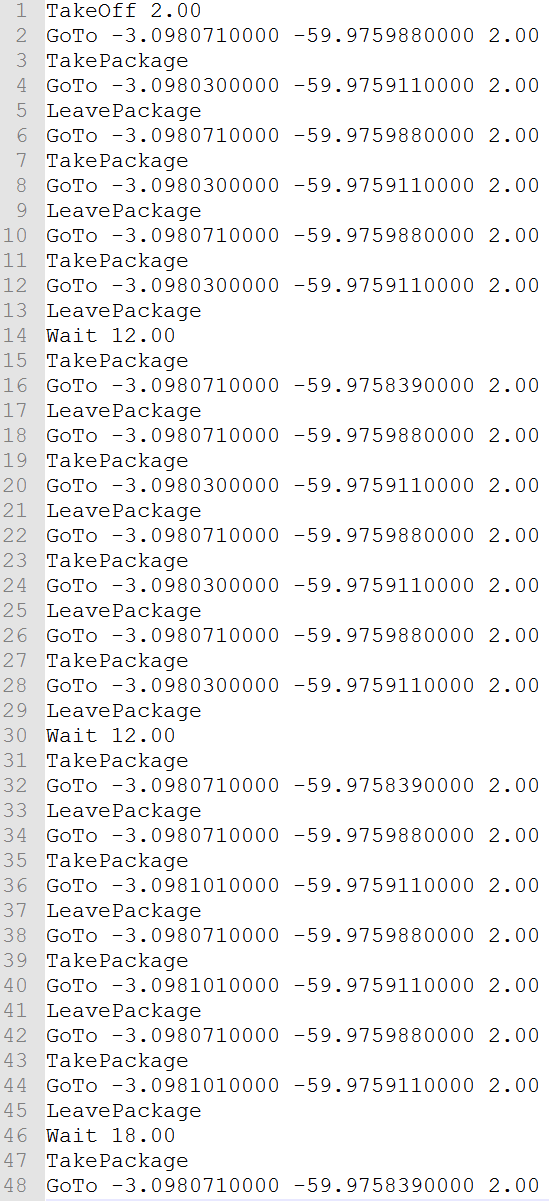
\includegraphics[width=.6\linewidth]{planAArq.PNG}
%  \caption{Planejador A.}
%  \label{fig:planAArq}
%\end{subfigure}%
%\begin{subfigure}{.5\textwidth}
%  \centering
%  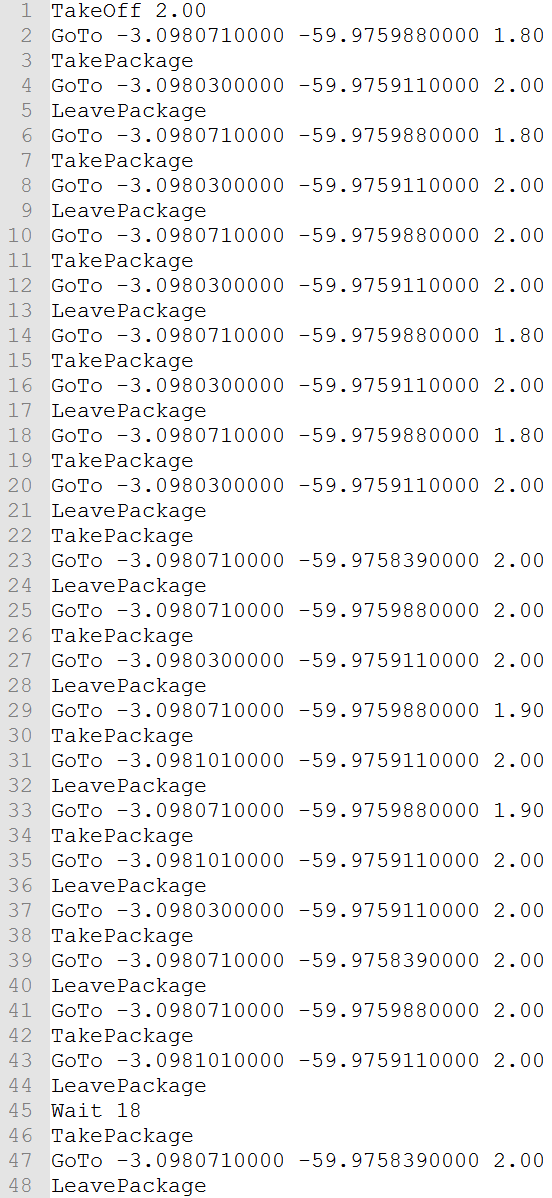
\includegraphics[width=.6\linewidth]{planBArq.PNG}
%  \caption{Planejador B.}
%  \label{fig:planBArq}
%\end{subfigure}
%\caption{Arquivos de Missão.}
%\label{fig:planArq}
%\end{figure}

%The two mission files shown above, have exactly the same instances, that is, they have the same resources and have to perform the same mission that is to produce two products of type X and one of type Y. However, they execute the mission of Different way and have different performances. As discussed in Section~\ref{sec:acusto}, planner B has more \texttt{GoTo} commands than planner A (see Figure~\ref{fig:planArq}).

Table~\ref{table:plannersSimulado} presents the performance (total flight time) of both planners algorithms.
\begin{table}[H]
\scriptsize
\centering
%\begin{adjustbox}{max width=\textwidth}
%\resizebox{7cm}{!}{%
\begin{tabular}{@{}ccc@{}}
\cmidrule(l){2-3}
                                        & \cellcolor[HTML]{FF7774}\textbf{Planner A} & \cellcolor[HTML]{5FCE89}\textbf{Planner B} \\ \cmidrule(l){2-3} 
\cellcolor[HTML]{C0C0C0}\textbf{Tests} & \textit{\textbf{Flight Time (s)}}            & \textit{\textbf{Flight Time (s)}}            \\
\cellcolor[HTML]{C0C0C0}1               & 460,405                                       & 430,830                                       \\
\cellcolor[HTML]{C0C0C0}2               & 460,693                                       & 436,885                                       \\
\cellcolor[HTML]{C0C0C0}3               & 462,080                                       & 441,681                                       \\
\cellcolor[HTML]{C0C0C0}4               & 457,719                                       & 441,277                                       \\
\cellcolor[HTML]{C0C0C0}5               & 461,227                                       & 451,865                                       \\ \bottomrule
\end{tabular}%
%}
%\end{adjustbox}
\caption{Mission Planners Flight Time - Simulator.\label{table:plannersSimulado}}
\end{table}

Table~\ref{table:plannersSimulado} indicates that the mission time of planner B is lower then the time of planner A in all five tests, ensuring the results of the evaluation methodology. Figure~\ref{fig:GraPlannersSimulado} shows a bar graph of the simulation flight times of both planners in the five tests.

\begin{figure}[H]
	\centering
	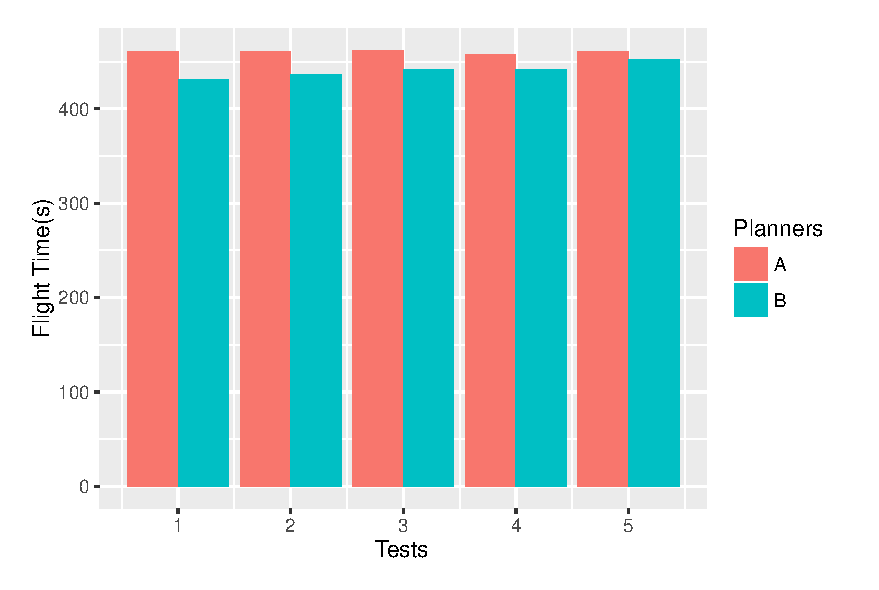
\includegraphics[width=0.7\columnwidth]{GraPlannersSimulado.eps}
	\caption{Flight Time Graph of Mission Planners Relative to 5 Tests in Simulator.\label{fig:GraPlannersSimulado}}
	\end{figure}
	
Additional experiments are performed with the real UAV system (3DR IRIS+). Figure~\ref{fig:maps} shows the map of experimental environment (Faculty of Physical Education and Physiotherapy of Federal University of Amazonas).

		\begin{figure}[H]
	\centering
	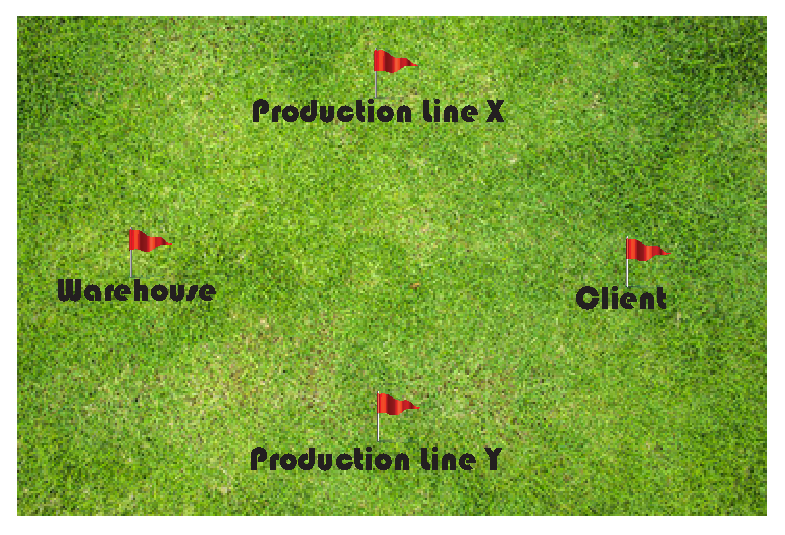
\includegraphics[width=0.7\columnwidth]{map.eps}
	\caption{Warehouse, Production Line X, Production Line Y and Costumer in the Map.\label{fig:maps}}
	\end{figure}
	
Table~\ref{table:plannersReal} shows the the flight times for both planners. The results indicates that the planner B also shown a shorter time compared to planner A in real environment.
	
	\begin{table}[H]
\scriptsize
\centering
%\resizebox{7cm}{!}{%
\begin{tabular}{@{}ccc@{}}
\cmidrule(l){2-3}
                                        & \cellcolor[HTML]{FF7774}\textbf{Planner A} & \cellcolor[HTML]{5FCE89}\textbf{Planner B} \\ \cmidrule(l){2-3} 
\cellcolor[HTML]{C0C0C0}\textbf{Tests} & \textit{\textbf{Flight Time (s)}}            & \textit{\textbf{Flight Time (s)}}            \\
\cellcolor[HTML]{C0C0C0}1               & 455,12                                       & 441,72                                       \\
\cellcolor[HTML]{C0C0C0}2               & 456,93                                       & 440,18                                       \\
\cellcolor[HTML]{C0C0C0}3               & 457,19                                       & 447,51                                      \\
\cellcolor[HTML]{C0C0C0}4               & 460,25                                       & 438,19                                       \\
\cellcolor[HTML]{C0C0C0}5               & 459.47                                       & 445,85                                       \\ \bottomrule
\end{tabular}%
%}
\caption{Mission Planners Flight Time - Real.\label{table:plannersReal}}
\end{table}

Figure~\ref{fig:GraPlannersReal} shows a bar graph of the flight times of both planners in the five tests with IRIS+.

\begin{figure}[H]
	\centering
	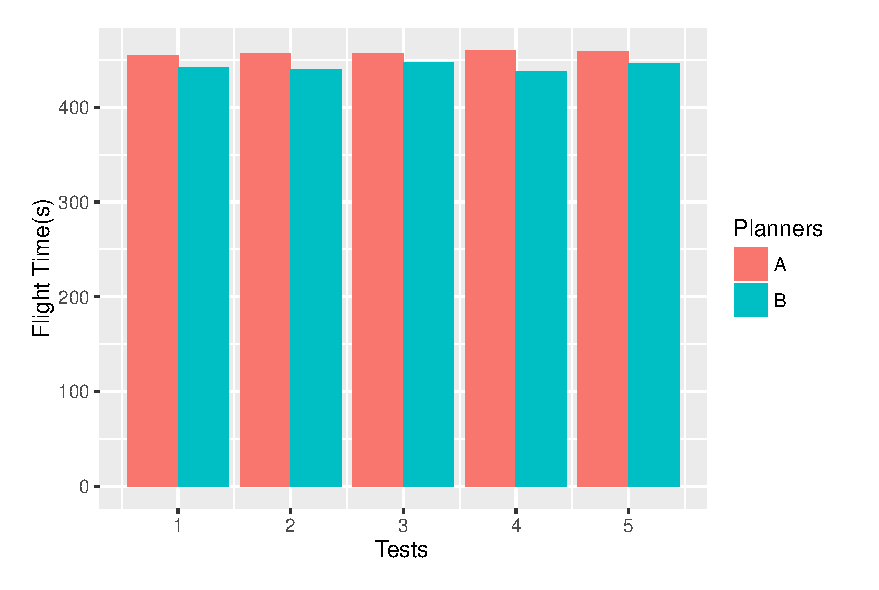
\includegraphics[width=0.7\columnwidth]{GraPlannersReal.eps}
	\caption{Flight Time Graph of Mission Planners Relative to 5 Tests in a Real Environment.\label{fig:GraPlannersReal}}
	\end{figure}
	
	The aforementioned results confirmed the prediction provided by the planner evaluation methodology, and the planner B is faster than planner A in all the tests with simulations and IRIS+ tests.
	
\subsection{Threats to Validity}
\label{sec:ameacas}

In order to compile the experiments, we have assembled a favourable environment to apply our evaluation metrics. In this way, we considered the use case in Section~\ref{sec:method}.

However, in case we change the scenario where the number of UAVs increases, our algorithms will not work as expected because we did not adapted the algorithms for cooperative work and consequently our metrics will not work as expected. Further works may be implemented to make the metrics works in a cooperative work environment where the number of UAVs is greater than two.

%\textcolor{red}{Thiago, nao ficou claro pra mim os objetivos dos experimentos... poderias escrever claramente quais seriam as research questions que devemos responder nos experimentos? Alem disso, precisas descrever uma secao sobre ameacas da validade dos resultados... como exemplo, olhe este artigo: https://arxiv.org/pdf/1610.04761.pdf}

%---------------------------------
\section{Conclusions}
\label{sec:conclusao}
%---------------------------------

We have presented an evaluation methodology for UAV mission planner in an industrial production scenario, as described in Section~\ref{sec:method}. We have used a evaluation methodology to perform two different algorithms to verify the performance of them. Our approach uses an optimizer tool to generate an optimal cost for a mission (w.r.t. flight time) and compares to different algorithm strategies using the index defined in Eq.~\ref{eq:MPCI}.
 
In addition, we have developed a framework for mission planning, command and control for intralogistics mission using a commercial UAV. Weused an UAV to solve intralogistics problems using the dronekit API to control and command adopting a high-level programming language.

Summary, our experiments to test the evaluation methodology for mission planner were done successfully as expected in simulated environment as well as in a real environment using a real UAV, and consequently, the methodology is able to evaluate mission planner algorithms for intralogistics problems. Moreover, the framework can solve the necessity of control and command a commercial UAV. Thus, our work is a new tool to verify a specific problem of intralogistics.

Future work includes the use of computational vision for the recognition of inputs, and improvements of the optimization problem modeling for better results in cost evaluation. Supplementary, we will make experiments in a cooperative work environment where the number of UAVs is greater than two.

%\selectlanguage{brazil}
%
%\section{Como utilizar o estilo \SBATeX}
%Este texto serve de guia de utilização do estilo \SBATeX para
%\LaTeXe. Com este estilo é possível gerar artigo no formato utilizado pelo \emph{Congresso
%  Brasileiro de Automática} e \emph{Simpósio Brasileiro de Automação Inteligente} na produção das versões acabadas dos artigos
%  nos anais.
%
%O seguinte parâmetro deve ser passado (entre colchetes) como argumento do comando
%\verb+\documentclass+, que deve ser o primeiro comando a aparecer no
%artigo. Por exemplo, o comando
%\begin{verbatim}
%  \documentclass[conference]{sbatex}
%\end{verbatim}
%é utilizado no início deste arquivo para geração do formato final
%para o \emph{Congresso Brasileiro de Automática} e o
%\emph{Simpósio Brasileiro de Automação Inteligente}.
%
%Pode-se adicionar ao comando \verb+\documentclass+ a seguinte
%opção:
%\begin{itemize}
%  \item \verb+harvard+: inclui o pacote \verb+harvard+, utilizado para
%  produção das referências bibliográficas. Pode ser usado em conjunto
%  com qualquer das outras opções. Veja seção~\ref{sec:bibliografia}.
%\end{itemize}
%Por exemplo, para propor um artigo ao congresso e utilizar o pacote de
%referências bibliográficas \verb+harvard+ usa-se o comando
%\begin{verbatim}
%  \documentclass[conference,harvard]{sbatex}
%\end{verbatim}
%A ordem dos parâmetros não é relevante.
%
%Os seguintes \emph{pacotes} \LaTeX\ estão disponíveis
%automaticamente\footnote{Isto também significa que \emph{é necessário
%ter estes pacotes instalados} para que se possa utilizar o estilo
%\SBATeX.} com o estilo \SBATeX:
%\begin{itemize}
%\item \verb+ifthen+: pacote com comandos de controle de fluxo do tipo
%`if', `then' e `else'; utilizado internamente para controle das opções de
%formatação.
%\item \verb+fancyhdr+: pacote para formatação dos cabeçalhos e rodapés.
%\item \verb+babel+: pacote para escrita em múltiplos idiomas; os
%idiomas/dialetos \verb+english+, \verb+brazil+ e \verb+spanish+ já
%estão habilitados.
%\item \verb+theorem+: pacote para controle dos ambientes \verb+theorem+,
%\verb+lemma+, \verb+corollary+ e \verb+proof+.
%\item \verb+geometry+: pacote para controle da dimensões do texto na página.
%\item \verb+latexsym+: pacote com símbolos extras do \LaTeXe.
%\end{itemize}
%
%A opção \verb+submission+ provê o pacote:
%\begin{itemize}
%\item \verb+setspace+: pacote para controle de espaçamento duplo entre
%linhas.
%\end{itemize}
%E a opção \verb+harvard+ provê o pacote:
%\begin{itemize}
%\item \verb+harvard+: pacote para formatação das referências
%bibliográficas.
%\end{itemize}
%
%Não é necessário incluir explicitamente as cláusulas
%\verb+\usepackage+ correspondentes a estes pacotes no artigo para que
%se possa utilizá-los. Caso a instalação do \LaTeX\ não contenha alguns
%destes pacotes, consulte a página
%\begin{verbatim}
%  http://www.ctan.org
%\end{verbatim}
%
%
%
%Com a opção \verb+conference+, e devido à escolha de um conjunto de
%fontes diferentes, recomenda-se subsituir o pacote \verb+fontenc+ pelo
%pacote \verb+ae+ (\emph{Almost European Computer Modern}), o que pode
%ser feito com o comando
%\begin{verbatim}
%  \usepackage{ae}
%\end{verbatim}
%Neste caso não é necessário adicionar explicitamente o pacote
%\verb+fontenc+, que já é carregado automaticamente pelo pacote
%\verb+ae+. Veja também a seção~\ref{sec:esqueleto}.
%
%Após o preâmbulo, inicia-se o texto propriamente dito por meio do
%comando
%\begin{verbatim}
%  \begin{document}
%\end{verbatim}
%O passo seguinte é a declaração do título do artigo, autores e
%afiliações.
%
%\subsection{Título, autores e afiliações}
%
%O título do artigo é declarado por meio do comando \verb+\title+. Por
%exemplo, o título deste artigo foi gerado com o comando:
%\begin{verbatim}
%  \title{Artigo Exemplo}
%\end{verbatim}
%O título não deve conter agradecimentos, os quais devem aparecer em
%uma seção separada, no final do artigo.
%
%Em seguida, definem-se os autores com seus endereços eletrônicos e
%afiliações por meio dos comandos \verb+\author+ e
%\verb+\address+. Por exemplo, o nome e endereço do primeiro autor
%deste artigo, João da Silva, é introduzido por meio dos comandos:
%\begin{verbatim}
%  \author{João da Silva}
%         {jsilva@silva.com}
%  \address{Endereço do João e da Maria\\
%           Em algum lugar\\
%           Cidade, Estado, País}
%\end{verbatim}
%Note-se que o comando \verb+\author+ requer dois argumentos: o nome e
%o endereço eletrônico. Quebras de linha podem ser obtidas na afiliação
%por meio do comando~\verb+\\+. Segue-se, neste exemplo, a declaração
%do nome e afiliação do segundo autor:
%\begin{verbatim}
%  \author{Joaquim Pereira}
%         {jpereira@pereira.org}
%  \address{Endereço do Joaquim\\
%           Em algum lugar\\
%           Cidade, Estado, País}
%\end{verbatim}
%
%Em geral, para cada comando \verb+\author+ deve haver um comando
%\verb+\address+ correspondente, salvo o caso de compartilhamento
%de endereços. Neste caso, omite-se o comando \verb+\address+ para
%o segundo autor e indica-se o número do endereço que se deseja
%compartilhar como um parâmetro adicional do comando
%\verb+\author+. Por exemplo, o comando:
%\begin{verbatim}
%  \author[1]{Maria da Silva}
%            {maria@pereira.org}
%\end{verbatim}
%indica que a Maria da Silva utilizará o endereço de número 1, que
%corresponde ao endereço de João da Silva.
%
%Os autores seguintes possuem endereços independentes e são
%introduzidos da maneira convencional:
%\begin{verbatim}
%  \author{Pedro Manoel}
%         {pedro@pedro.com}
%  \address{Endereço do Pedro e do Rafael\\
%           Em algum lugar\\
%           Cidade, Estado, País}
%
%  \author{José Rodrigues}
%         {jose@rodrigues}
%  \address{Endereço do José\\
%           Em algum lugar\\
%           Cidade, Estado, País}
%\end{verbatim}
%
%Finalmente, o autor Rafael é definido como
%\begin{verbatim}
%  \author[3]{Rafael Pires}
%            {rafael@pires}
%\end{verbatim}
%o que indica que Rafael compartilha o endereço de número 3 com Pedro
%Manoel. Lembre-se de que, apesar de Pedro Manoel ser o autor de número
%4, o seu endereço é o de número 3, uma vez que a Maria já compartilha
%-- sem segundas intenções -- do mesmo endereço com o João.
%
%O comando
%\begin{verbatim}
%  \maketitle
%\end{verbatim}
%coloca o título e os autores no formato adequado.
%
%
%\subsection{Resumo, abstract e palavras-chave}
%
%Os artigos devem conter um resumo em português (ou espanhol) e em
%inglês. O ambiente para definição dos resumos, em qualquer idioma, é o
%\verb+abstract+. Para diferenciar os idiomas utiliza-se o comando
%\verb+\selectlanguage+, do pacote \verb+babel+. Por exemplo, a seqüência
%de comandos produz um \emph{Abstract} seguido de um \emph{Resumo}:
%\begin{verbatim}
%  \selectlanguage{english}
%  \begin{abstract}
%    Yossarian says, ...
%  \end{abstract}
%
%  \selectlanguage{brazil}
%  \begin{abstract}
%    O Largo da Sé ...
%  \end{abstract}
%\end{verbatim}
%
%As \emph{palavras-chave} devem ser definidas por meio do comando:
%\begin{verbatim}
%  \keywords{Exemplo, Ilustração}
%\end{verbatim}
%
%Deste ponto em diante selecione o idioma a ser utilizado e
%inicie o texto da sua contribuição.
%
%\textbf{IMPORTANTE:} Caso esteja se produzindo um texto com a
%opção \verb+conference+, colocam-se os comandos que vão de
%\verb+\maketitle+ a \verb+\keywords+ dentro de um ambiente
%\verb+twocolumn+. Isto é necessário para que os resumos sejam
%formatados em coluna simples\footnote{Como este arquivo está
%adaptado para utilizar o formato adequado para o \emph{Congresso
%Brasileiro de Automática} e o \emph{Simpósio Brasileiro de
%Automação Inteligente}, isto já está feito}. Veja
%seção~\ref{sec:esqueleto}.
%
%
%\subsection{Teoremas, lemas, corolários e provas}
%
%Quatro ambientes já se encontram pré-definidos no estilo \SBATeX. São
%eles
%\begin{itemize}
%\item \verb+theorem+: ambiente para teoremas.
%\item \verb+corollary+: ambiente para corolários.
%\item \verb+lemma+: ambiente para lemas.
%\item \verb+proof+: ambiente para provas.
%\end{itemize}
%Segue-se um exemplo de utilização destes ambientes:
%\begin{lemma}[Desigualdade Subtrativa]
%Em um espaço vetorial linear normado $\|x\| - \|y\| \leq \|x - y\|$
%para quaisquer vetores $x$, $y$.
%\end{lemma}
%\begin{proof}
%\begin{align*}
%\|x\| - \|y\| &= \|x - y + y\| - \|y\| \ \\
%              &\leq \|x - y \| + \|y\| - \|y\| \\
%              &= \|x - y\|.
%\end{align*}
%\end{proof}
%Este lema é produzido pela seguinte sequência de comandos:
%\begin{verbatim}
%  \begin{lemma}[Desigualdade Subtrativa]
%    Em um espaço vetorial linear ...
%  \end{lemma}
%  \begin{proof}
%    ...
%  \end{proof}
%\end{verbatim}
%
%Estes ambientes, com exceção do ambiente \verb+proof+, aceitam
%um parâmetro opcional que define um nome. No exemplo acima, o nome
%\emph{Desigualdade Subtrativa} foi produzido por meio deste argumento.
%
%
%\subsection{Bibliografia}
%\label{sec:bibliografia}
%
%As referências são reunidas ao fim do manuscrito, arranjadas
%alfabeticamente pelo primeiro autor e cronologicamente para cada
%autor.
%
%\textbf{IMPORTANTE:} Todas referências citadas devem aparecer em algum
%outro ponto do texto.
%
%As citações seguem um estilo autor/ano (o mesmo
%usado na revista {\em Automatica}). O pacote \verb+harvard+ (já
%incluído pelo \SBATeX) provê vários comandos para inclusão de
%citações. Dois dois mais utilizados são o tradicional \verb+\cite+ e o
%\verb+\citeasnoun+. Veja um exemplo:
%\begin{verbatim}
%  O resumo deste artigo é um trecho do
%  livro~\citeasnoun{serafim}. Já o abstract é
%  extraído de~\citeasnoun{catch22}.
%  Informações sobre o estilo bibliográfico
%  \verb+harvard+ encontram-se
%  em~\citeasnoun{harvard}. Os interessados
%  devem consultar referências adicionais
%  sobre \LaTeX~\cite{latex,%
%  latex:guide,latex:companion}.
%\end{verbatim}
%produz o trecho:
%
%\begin{em}
%  O resumo deste artigo é um trecho do
%  livro~\citeasnoun{serafim}. Já o abstract é
%  extraído de~\citeasnoun{catch22}.
%  Informações sobre o estilo bibliográfico
%  \verb+harvard+ encontram-se
%  em~\citeasnoun{harvard}. Os interessados
%  devem consultar referências adicionais
%  sobre \LaTeX~\cite{latex,latex:guide,latex:companion}.
%\end{em}
%
%Recomenda-se a utilização do programa BibTeX para gerar as suas
%referências ~\cite{latex,latex:guide,latex:companion}. Note-se que
%não é necessário definir o estilo bibliográfico com o comando
%\verb+\bibliographystyle+, pois o mesmo é definido automaticamente
%pelo estilo \SBATeX. Basta incluir o arquivo de bibliografias,
%neste exemplo o artigo \verb+exemplo.bib+ por meio do comando.
%\begin{verbatim}
%    ...
%
%    \bibliography{exemplo}
%
%  \end{document}
%\end{verbatim}
%Note-se que este comando deve ser colocado logo antes do
%encerramento do artigo, o que é feito pelo comando
%\verb+\end{document}+, de tal forma a garantir que a bibliografia
%seja o último item do artigo.
%
%
%\subsection{Esqueleto deste arquivo no formato \SBATeX}
%\label{sec:esqueleto}
%
%Este arquivo, adaptado para gerar o formato adequado para o
%\emph{Congresso Brasileiro de Automática} e o  \emph{Simpósio
%Brasileiro de Automação Inteligente}, faz uso da seguintes
%instruções:
%
%\begin{verbatim}
%\documentclass[conference,harvard,brazil,english]{sbatex}
%  \usepackage[utf8]{inputenc}
%  \usepackage{ae}
%
%    ...
%
%    \twocolumn[
%      \maketitle
%
%      \selectlanguage{english}
%      \begin{abstract}
%        Yossarian says, ...
%      \end{abstract}
%
%      \selectlanguage{brazil}
%      \begin{abstract}
%        O Largo da Sé ...
%      \end{abstract}
%
%      \keywords{Exemplo, Ilustração}
%    ]
%
%    ...
%\end{verbatim}
%
%
%\section{Contribuição deste artigo}
%
%\subsection{Os vinte e sete erros mais comuns (de uma lista de cem)}
%\label{sec:27erros}
%
%Erros gramaticais e ortográficos devem, por princípio, ser
%evitados. Alguns, no entanto, como ocorrem com maior frequência,
%merecem atenção redobrada. O primeiro capítulo deste manual inclui
%explicações mais completas a respeito de cada um deles. Veja os cem
%mais comuns do idioma e use esta relação como um roteiro para fugir
%deles~\cite{manual}.
%
%\begin{enumerate}
%\item ``Mal cheiro'', ``mau-humorado''. Mal opõe-se a bem e mau, a
%bom. Assim: mau cheiro (bom cheiro), mal-humorado
%(bem-humorado). Igualmente: mau humor, mal-intencionado, mau jeito,
%mal-estar.
%
%\item ``Fazem'' cinco anos. Fazer, quando exprime tempo, é impessoal:
%Faz cinco anos.~/~Fazia dois séculos.~/~Fez 15 dias.
%
%\item ``Houveram'' muitos acidentes. Haver, como existir, também é
%invariável: Houve muitos acidentes.~/~Havia muitas pessoas.~/~Deve
%haver muitos casos iguais.
%
%\item ``Existe'' muitas esperanças. Existir, bastar, faltar, restar e
%sobrar admitem normalmente o plural: Existem muitas esperanças. /
%Bastariam dois dias.~/~Faltavam poucas peças.~/~Restaram alguns
%objetos.~/~Sobravam idéias.
%
%\item Para ``mim'' fazer. Mim não faz, porque não pode ser
%sujeito. Assim: Para eu fazer, para eu dizer, para eu trazer.
%
%\item Entre ``eu'' e você. Depois de preposição, usa-se mim ou ti: Entre
%mim e você.~/~Entre eles e ti.
%
%\item ``Há'' dez anos ``atrás''. Há e atrás indicam passado na frase. Use
%apenas há dez anos ou dez anos atrás.
%
%\item ``Entrar dentro''. O certo: entrar em. Veja outras redundâncias:
%Sair fora ou para fora, elo de ligação, monopólio exclusivo, já não há
%mais, ganhar grátis, viúva do falecido.
%
%\item ``Venda à prazo''. Não existe crase antes de palavra masculina, a
%menos que esteja subentendida a palavra moda: Salto à (moda de) Luís
%XV. Nos demais casos: A salvo, a bordo, a pé, a esmo, a cavalo, a
%caráter.
%
%\item ``Porque'' você foi? Sempre que estiver clara ou implícita a
%palavra razão, use por que separado: Por que (razão) você foi?~/~Não
%sei por que (razão) ele faltou.~/~Explique por que razão você se
%atrasou. Porque é usado nas respostas: Ele se atrasou porque o
%trânsito estava congestionado.
%
%\item Vai assistir ``o'' jogo hoje. Assistir como presenciar exige a:
%Vai assistir ao jogo, à missa, à sessão.  Outros verbos com a: A
%medida não agradou (desagradou) à população.~/~Eles obedeceram
%(desobedeceram) aos avisos.~/~Aspirava ao cargo de diretor.~/~Pagou ao
%amigo.~/~Respondeu à carta.~/~Sucedeu ao pai.~/~Visava aos estudantes.
%
%\item Preferia ir ``do que'' ficar. Prefere-se sempre uma coisa a outra:
%Preferia ir a ficar. É preferível segue a mesma norma: É preferível
%lutar a morrer sem glória.
%
%\item O resultado do jogo, não o abateu. Não se separa com vírgula o
%sujeito do predicado. Assim: O resultado do jogo não o abateu. Outro
%erro: O prefeito prometeu, novas denúncias. Não existe o sinal entre o
%predicado e o complemento: O prefeito prometeu novas denúncias.
%
%\item Não há regra sem ``excessão''. O certo é exceção. Veja outras
%grafias erradas e, entre parênteses, a forma correta: ``paralizar''
%(paralisar), ``beneficiente'' (beneficente), ``xuxu'' (chuchu),
%``previlégio'' (privilégio), ``vultuoso'' (vultoso), ``cincoenta''
%(cinqüenta), ``zuar'' (zoar), ``frustado'' (frustrado), ``calcáreo''
%(calcário), ``advinhar'' (adivinhar), ``benvindo'' (bem-vindo), ``ascenção''
%(ascensão), ``pixar'' (pichar), ``impecilho'' (empecilho), ``envólucro''
%(invólucro).
%
%\item Quebrou ``o'' óculos. Concordância no plural: os óculos, meus
%óculos. Da mesma forma: Meus parabéns, meus pêsames, seus ciúmes,
%nossas férias, felizes núpcias.
%
%\item Comprei ``ele'' para você. Eu, tu, ele, nós, vós e eles não podem
%ser objeto direto. Assim: Comprei-o para você. Também: Deixe-os sair,
%mandou-nos entrar, viu-a, mandou-me.
%
%\item Nunca ``lhe'' vi. Lhe substitui a ele, a eles, a você e a vocês e
%por isso não pode ser usado com objeto direto: Nunca o vi.~/~Não o
%convidei.~/~A mulher o deixou.~/~Ela o ama.
%
%\item ``Aluga-se'' casas. O verbo concorda com o sujeito: Alugam-se
%casas.~/~Fazem-se consertos.~/~É assim que se evitam acidentes. /
%Compram-se terrenos.~/~Procuram-se empregados.
%
%\item ``Tratam-se'' de. O verbo seguido de preposição não varia nesses
%casos: Trata-se dos melhores profissionais.~/~Precisa-se de
%empregados.~/~Apela-se para todos.~/~Conta-se com os amigos.
%
%\item Chegou ``em'' São Paulo. Verbos de movimento exigem a, e não em:
%Chegou a São Paulo.~/~Vai amanhã ao cinema.~/~Levou os filhos ao
%circo.
%
%\item Atraso implicará ``em'' punição. Implicar é direto no sentido de
%acarretar, pressupor: Atraso implicará punição.~/~Promoção implica
%responsabilidade.
%
%\item Vive ``às custas'' do pai. O certo: Vive à custa do pai. Use
%também em via de, e não ``em vias de'': Espécie em via de extinção. /
%Trabalho em via de conclusão.
%
%\item Todos somos ``cidadões''. O plural de cidadão é cidadãos. Veja
%outros: caracteres (de caráter), juniores, seniores, escrivães,
%tabeliães, gângsteres.
%
%\item O ingresso é ``gratuíto''. A pronúncia correta é gratúito, assim
%como circúito, intúito e fortúito (o acento não existe e só indica a
%letra tônica). Da mesma forma: flúido, condôr, recórde, aváro, ibéro,
%pólipo.
%
%\item A última ``seção'' de cinema. Seção significa divisão, repartição,
%e sessão equivale a tempo de uma reunião, função: Seção Eleitoral,
%Seção de Esportes, seção de brinquedos; sessão de cinema, sessão de
%pancadas, sessão do Congresso.
%
%\item Vendeu ``uma'' grama de ouro. Grama, peso, é palavra masculina: um
%grama de ouro, vitamina C de dois gramas. Femininas, por exemplo, são
%a agravante, a atenuante, a alface, a cal, etc.
%
%\item ``Porisso''. Duas palavras, por isso, como de repente e a partir
%de.
%
%\end{enumerate}
%
%\subsection{Observação importante}
%
%Os erros de português porventura presentes neste artigo
%\begin{itemize}
%\item ou foram introduzidos propositalmente para deleite dos leitores
%atentos,
%\item ou não constam da lista da seção~\ref{sec:27erros}.
%\end{itemize}
%
%\section{Conclusões}
%Nada resta senão desejar-lhe boa sorte na preparação de seu artigo. Contamos com seu trabalho e sua presença no SBAI 2017 a ser realizado em Porto Alegre-RS.
%
%\section*{Agradecimentos}
%Mencione aqui seus agradecimentos as agências de fomento e colaboradores no trabalho.


\selectlanguage{english}
% BIBLIOGRAFIA
\bibliography{exemplo}
\end{document}
